%--------------------------------------------------
\section{Scan of Jet Energy Scale in the fit}
The main uncertainty in jet reconstruction comes from the jet energy
scale (JES) uncertainty.  A
preliminary estimate from 2010 data showed that the jet energy
uncertainty could be kept within 4\% and the jet resolution
uncertainty within 10\%.  For more details, see
Refs.~\cite{jetsyst,jetsyst2}.  The systematic uncertainties in the
JES and jet resolution affect the signal acceptance and
the $m_{jj}$ distribution.

The fitter therefore contained a free parameter ($JES_{shift}$) to
parametrize the difference between the Monte Carlo and the data. This
difference could vary along a Gaussian with a $\sigma=0.05m_{jj}$. The
most direct way to estimate the associated systematic uncertainty is
to compare the results of the fit where $JES_{shift}$ is allowed to
float versus requiring $JES_{shift}=0$. Implementing this procedure
gave an error in the WW-Yield $\leq 5\% $. In addition we verified that
the fit is stable and returns the best ({\it i.e.} consistent with the
minimum $\chi^2$) value by assigning $JES_{shift}$ fixed values from
$-0.05m_{jj}$ to $+0.05m_{jj}$ and repeating the fit. The results are
given in Table~\ref{table:JESScanResults} with $\chi^2$ shown in
Figure~\ref{fig:JESScanchi2}. The minimum in $\chi^2$ is consistent
with the value obtained when the $JES_{shift}$ is allowed to float
($0.003m_{jj}$) and the fit has a stable, well defined minimum. Note
that the above study serves a crosscheck, since we use the Ws from top
quark events to estimate the JES uncertainty (Section.~\ref{sec:topw}).

%%%%%%%%%%%%
\begin{table}[tb]
\caption{\sl $JES_{shift}$ Scan Crosscheck}
\begin{center}
\begin{tabular}{|c|c|c|}
\hline
   $JES_{shift}/m_{jj}$
 & WW-Yield
 & $\chi^2$ \cr
\hline
\vspace{-0.5cm} & & \cr
{$-0.05$} & $1012$ & $3.77$  \cr
\hline
{$-0.04$} & $960$ & $2.84$  \cr
\hline
{$-0.03$} & $901$ & $2.01$  \cr
\hline
{$-0.02$} & $874$ & $1.49$  \cr
\hline
{$-0.01$} & $877$ & $1.10$  \cr
\hline
{$0.0$} & $793$ & $0.95$  \cr
\hline
{$0.01$} & $676$ & $0.86$  \cr
\hline
{$0.02$} & $594$ & $0.95$  \cr
\hline
{$0.03$} & $496$ & $1.17$  \cr
\hline
{$0.04$} & $354$ & $1.61$  \cr
\hline
{$0.05$} & $261$ & $2.09$  \cr
\hline
\end{tabular}
\end{center}
\label{table:JESScanResults}
\end{table}
%%%%%%%%%%%%
\begin{figure}[h!] {\centering
    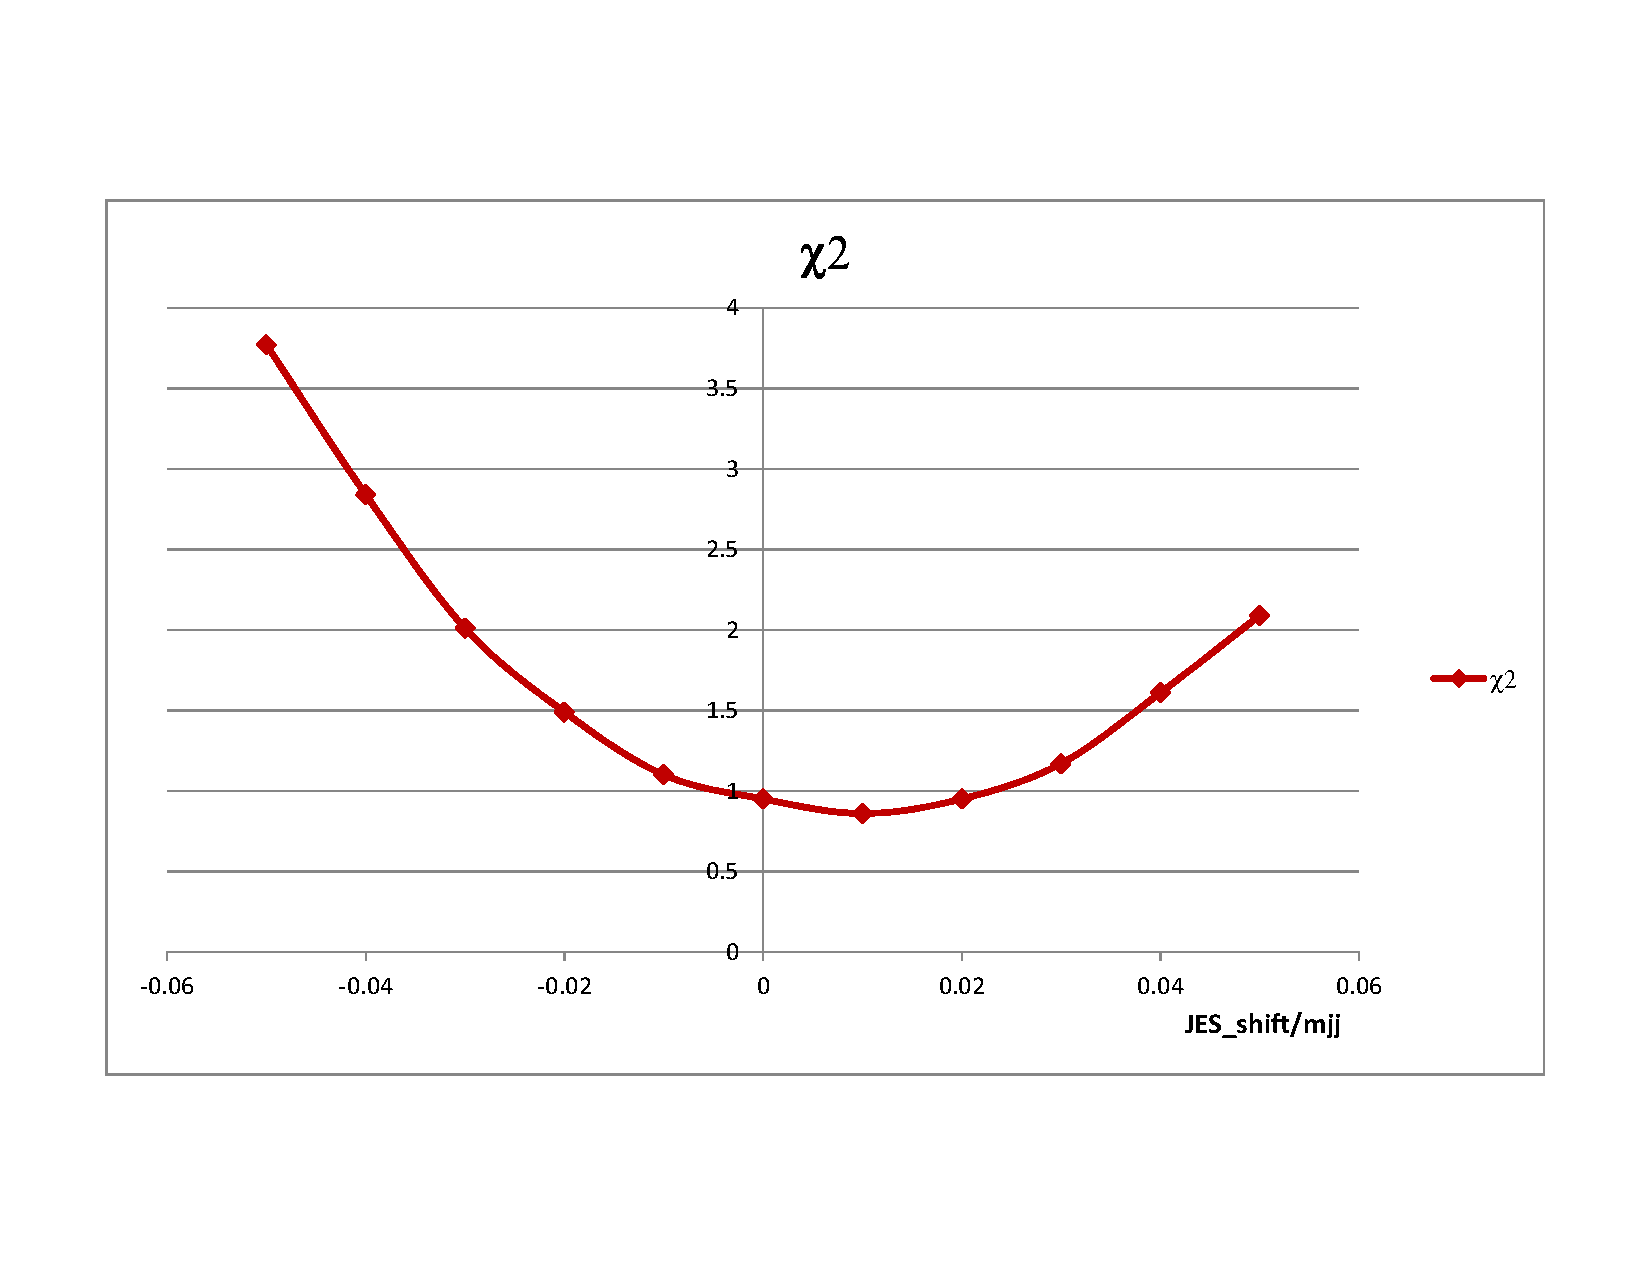
\includegraphics[width=0.5\textwidth]{figs/JES_scan.pdf}
    \caption{$\chi^2$ of the fit vs $JES_{shift}/m_{jj}$.}
    \label{fig:JESScanchi2}}
\end{figure}
%%%%%%%%%%%%